\documentclass{article}
\usepackage{epsfig, latexsym}

\begin{document}

\newcommand{\SOPmin}{${\rm SOP}_{\rm min} \ $}
\newcommand{\POSmin}{${\rm POS}_{\rm min} \ $}
\newcommand{\bs}{\backslash}


\title{
\Huge{CSE 271 -- Fall 2000}\\
\normalsize{Exam 3}\\
\normalsize{Return this document!!!}\\
\makebox[4in][l]{Name:}
SSN:}
\date{}

\maketitle{}

\begin{enumerate}
\item {\bf (3 pts.)} How many \SOPmin realizations does F have?
F(A,B,C,D)=$\Sigma$m(0,1,2,5,6,8,11,12,15)
\marginpar{ \tiny $$ \begin{array} {c||c|c|c|c}
        AB \bs CD & 00 & 01 & 11 & 10 \\ \hline \hline
        00        &    &    &    &    \\ \hline
        01        &    &    &    &    \\ \hline
        11        &    &    &    &    \\ \hline
        10        &    &    &    &    \\
\end{array} $$ }

\begin{tabular}{p{0.75in}p{0.75in}p{0.75in}p{0.75in}p{0.75in}}
a) 1 & b) 2 & c) 3 & d) 4 & e) 5 \\
\end{tabular}

\item {\bf (3 pts.)} The output of a sequential circuit is fundamentally
different than a combinational circuit because its output is a function
of the?
\begin{description}
\item{a) } State
\item{b) } Input
\item{c) } Output
\item{d) } Number of inputs
\item{e) } The staple monkey
\end{description}

\item {\bf (3 pts.)} A Moore-type FSM has been implemented using D flip
flops.  Your manager wants you to explore the cost associated with
a T flip flop realization.  Which FSM design steps need to be redone?
\begin{description}
\item{a) } Memory input equations.
\item{b) } Memory input equations and output equations.
\item{c) } Transition kmap, memory input equations and output equations.
\item{e) } Trick questions, all steps of the design must be re-performed.
\item{e) } Trick questions, none of the steps need to be redone.  Just 
insert T flip flops in place of the D flip flops.
\end{description}

\item {\bf (2 pts.)} You are told to implement a 3 bit counter using our seven
step FSM design process.  Each state represents the current count value.  The
binary representations of the states are assigned minimal length representations.
How many flip flops will this FSM require?

\begin{tabular}{p{0.75in}p{0.75in}p{0.75in}p{0.75in}p{0.75in}}
a) 3 & b) 4 & c) 7 & d) 8 & e) 16 \\
\end{tabular}

\item {\bf (2 pts.)} You are told to implement a 3 bit counter using the
ones hot design process.  Each state represents the current count value. 
How many flip flops will the counter require?

\begin{tabular}{p{0.75in}p{0.75in}p{0.75in}p{0.75in}p{0.75in}}
a) 3 & b) 4 & c) 7 & d) 8 & e) 16 \\
\end{tabular}

\item {\bf (1 pts.)} Large counters (e.g. 16 bit) are implemented using ones hot 
coding of the states.

\begin{tabular}{p{0.75in}p{0.75in}p{0.75in}p{0.75in}p{0.75in}}
a) True & b) False  &      &      &      \\
\end{tabular}

Questions 7-10 concern the FSM realization of the state diagram given below.
Assume a ones hot encoding.  Call the input X and the output Z.  Let $D_A$ 
be the input to the
flip flop representing state A.  Let $Q_A$ be the output from the flip flop 
representing state A.  Apply the preceding definitions to $D_B, Q_B, D_C, Q_C$.

\item {\bf (1 pts.)} How many flip flops are required to realize this FSM?

\begin{tabular}{p{0.75in}p{0.75in}p{0.75in}p{0.75in}p{0.75in}}
a) 1 & b) 2 & c) 3 & d) 4 & e) 4 \\
\end{tabular}

\item {\bf (3 pts.)} What is the memory input equation for flip flop {\bf A}?
\begin{description}
\item{a) } $XQ_C + XQ_A$
\item{b) } $X'Q_A$
\item{c) } $X'D_A$
\item{d) } $XD_C + XD_A$
\item{e) } None of the above.
\end{description}

\item {\bf (3 pts.)} What is the memory input equation for flip flop {\bf R}?
\begin{description}
\item{a) } 1
\item{b) } 0
\item{c) } $XQ_B + X'Q_C$
\item{d) } $XD_B + X'D_C$
\item{e) } None of the above.
\end{description}
\includegraphics[-60mm,15mm][0mm,15.1mm]{./Fig3/sd.eps}
\item {\bf (3 pts.)} What is the equation for Z?
\begin{description}
\item{a) } $X'Q_A + X'Q_B + X'Q_C$
\item{b) } $X'+Q_C$
\item{c) } $X'D_C + X'D_B + X'D_A$
\item{d) } $X' + D_C$
\item{e) } None of the above.
\end{description}
\pagebreak
Questions 11-15 deal with the construction of a 1Mx32 RAM using 64kx4
RAM chips and a decoder.

\item {\bf (2 pts.)} How many 64kx4 RAM chips are required to construct 
the 1Mx32 RAM?

\begin{tabular}{p{0.75in}p{0.75in}p{0.75in}p{0.75in}p{0.75in}}
a) 4 & b) 16 & c) 32 & d) 64 & e) 128 \\
\end{tabular}

\item {\bf (2 pts.)} How big is the decoder required to construct the 
1Mx32 RAM?

\begin{tabular}{p{0.75in}p{0.75in}p{0.75in}p{0.75in}p{0.75in}}
a) 2:4 & b) 3:8 & c) 4:16 & d) 5:32 & e) 6:64 \\
\end{tabular}

\item {\bf (2 pts.)} How many bits of address does each 64kx4 RAM chips have?

\begin{tabular}{p{0.75in}p{0.75in}p{0.75in}p{0.75in}p{0.75in}}
a) 4 & b) 16 & c) 64 & d) 16k & e) 64k \\
\end{tabular}

\item {\bf (2 pts.)} All the RE lines in a 64kx4 RAM chips are tied together.

\begin{tabular}{p{0.75in}p{0.75in}p{0.75in}p{0.75in}p{0.75in}}
a) True & b) False  &      &      &      \\
\end{tabular}

\item {\bf (2 pts.)} How many 64kx4 RAM chips get the MSB of the 32 bit data input?

\begin{tabular}{p{0.75in}p{0.75in}p{0.75in}p{0.75in}p{0.75in}}
a) 4 & b) 16 & c) 32 & d) 64 & e) 128 \\
\end{tabular}

For questions 16-18 assume that you have constructed a circuit
which is involved in a 2 line handshake; your circuit
is a passive consumer of data.  

\item {\bf (3 pts.)} Which of the following explanations justifies delaying 
acknowledgement until after you latch the data?
\begin{description}
\item{a) } The external world may be much faster than your circuit.
\item{b) } The external world may be much slower than your circuit.
\item{c) } The external world may be the same speed as your circuit.
\item{d) } The external world may be busy.
\item{e) } Our circuit may be busy.
\end{description}

\item {\bf (3 pts.)} The data given to our circuit, from the external
world, comes from a circuit called {\bf X}.  What role is {\bf X}
playing in the 2 line handshake?
\begin{description}
\item{a) } Active producer
\item{b) } Passive producer
\item{c) } Active consumer
\item{d) } Passive consumer
\end{description}

\item {\bf (3 pts.)} ACK...
\begin{description}
\item{a) } is a funny noise made by Martians.
\item{b) } is used by our circuit to affirm reception of data
\item{c) } stands for acknowledge.
\item{d) } is an output of our control unit.
\item{e) } All of the above.
\end{description}

\pagebreak
The following is part of an algorithm.  The corresponding piece of the
control unit is shown to the right.

\includegraphics[-60mm,50mm][0mm,51mm]{./Fig3/branch.eps}

\begin{verbatim}
if (x=1) then 
    if (y=1) then A=A+1;
    else          B=B+1;
else        
    if (y=1)      C=C+1;
    else          D=D+1;
\end{verbatim}
\vspace{16mm}


\item {\bf (3 pts.)} In which state does D get incremented?

\begin{tabular}{p{0.75in}p{0.75in}p{0.75in}p{0.75in}p{0.75in}}
a) S4 & b) S5 & c) S6 & d) S7 & e) other \\
\end{tabular}

\item {\bf (3 pts.)}Assume that X=1 and Y=1.  Given the partial timing 
diagram below, about what time will the outputs of the A register 
equal A+1?

\begin{tabular}{p{0.75in}p{0.75in}p{0.75in}p{0.75in}p{0.75in}}
a) 40nS & b) 60nS & c) 80nS & d) 120nS & e) 140nS \\
\end{tabular}

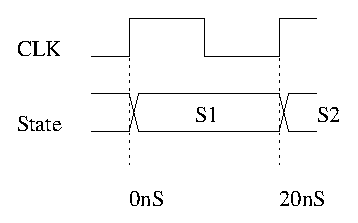
\includegraphics{./Fig3/time.eps}

\item {\bf (3 pts.)} How many states can the control unit be
reduced to, assuming that you keep state S1?

\begin{tabular}{p{0.75in}p{0.75in}p{0.75in}p{0.75in}p{0.75in}}
a) 1 & b) 4 & c) 5 & d) 6 & e) 7 \\
\end{tabular}

\pagebreak
Questions 22-46 (1 pt. each), 47-49 deal with the construction of a digital circuit to
accomplish a task specified by an algorithm.  A(0) refers to the LSB of A.
A $>>$ 1 refers to A shifted right 1 bit.

{\small
\begin{verbatim}
while(1) {
    while(REQ == 0);              // If the control bit equals 0 or 00  mark A 
    A = datainA;                  // If the control bit equals 01       mark B 
    B = datainB;                  // If the control bit equals 10       mark C 
    ACK = 1;                      // If the control bit equals 1 or 11  mark D 
    while (REQ == 1);             // If the control bit is a don't care mark E 
    ACK = 0;
    C = 0;
    for (i=0; i<B; i++) {
        if (A(0) == 1) then
            C = C + 1;
        else 
            C = C - 1;
        A = A >> 1;
}   } 
\end{verbatim}}
\begin{figure}[ht]
\centerline{\psfig{figure=./Fig3/dp&cu.eps,width=5in.,clip=}}
\end{figure}

\begin{tabular}{|l||l|l|l|l|l|l|l|}  \hline
State & ACK & A       & B      & C      & Mux        & count   & Add/Sub \\ \hline
      & 0   & 00 hold & 0 hold & 0 hold & 0 pass 0   & 00 hold & 0 add \\ \hline  
      & 1   & 01 SR   & 1 load & 1 load & 1 pass C$\pm$1 & 01 down & 1 sub \\ \hline  
      &     & 10 SL   &        &        &            & 10 up   &       \\ \hline  
      &     & 11 load &        &        &            & 11 load &       \\ \hline   \hline
Wait1 & 22  &         &        &        &            &         &       \\ \hline
Get   & 23  &  26     &  30    &  32    &  36        &  41     & 43    \\ \hline
Wait2 & 24  &  27     &        &        &  37        &  42     &       \\ \hline
For/If &    &         &        &        &            &         &       \\ \hline
Inc   &     &  28     &        &  33    &  38        &         & 44    \\ \hline
Dec   & 25  &         &        &  34    &  39        &         & 45    \\ \hline
Shift &     &  29     &  31    &  35    &  40        &         & 46    \\ \hline
\end{tabular}
\pagebreak
\setcounter{enumi}{46}
\item {\bf (3 pts.)} How many bits are in the status word?

\begin{tabular}{p{0.75in}p{0.75in}p{0.75in}p{0.75in}p{0.75in}}
a) 1 & b) 2 & c) 4 & d) 5 & e) 9 \\
\end{tabular}

\item {\bf (3 pts.)} Let A be N bits wide.  Let B's range be $[0,log_2(N)]$.
How many bits wide is the B register?

\begin{tabular}{p{1.30in}p{1.30in}p{2.00in}}
a) $log_2(log_2(N))$ & b) $log_2(log_2(N))+1$ &   \\
c) $log_2(N)$ & d) $log_2(N)+1$ & e) None of these.\\
\end{tabular}

\item {\bf (3 pts.)} Use the same assumptions about A and B as stated in the previous
problem.  How many bits wide does the C register need to be?

\begin{tabular}{p{1.30in}p{1.3in}p{2.00in}}
a) $log_2(log_2(N))+1$ & b) $log_2(N)+1$ &   \\
c) $N+1$ & d) $2^N+1$ & e) None of these.\\
\end{tabular}

Questions 50-52 deal with the following figure.  Assume that the
setup, hold, and propagation delay of the flip flops is 2 nS.
The combinational logic box has a propagation delay of 2nS.

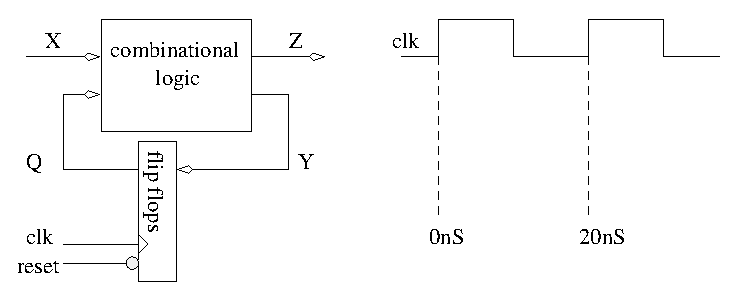
\includegraphics{./Fig3/fsm.eps}

\item {\bf (3 pts.)}Under what conditions will the circuit reset.
\begin{description}
\item{a) } When the clock rises and reset = 1.
\item{b) } When reset = 1.
\item{c) } When the clock rises and reset = 0.
\item{d) } When reset = 0.
\item{e) } None of the above.
\end{description}

\item {\bf (3 pts.)}Which of the following times does Q change?

\begin{tabular}{p{0.75in}p{0.75in}p{0.75in}p{0.75in}p{0.75in}}
a) 20nS  & b) 22nS  & c) 24nS & d) 26nS & e) 28nS \\
\end{tabular}

\item {\bf (3 pts.)}What is the latest time that X can be changed
without violating timing constraints?

\begin{tabular}{p{0.75in}p{0.75in}p{0.75in}p{0.75in}p{0.75in}}
a) 32nS  & b) 34nS  & c) 36nS & d) 38nS & e) 40nS \\
\end{tabular}
%% This is an ABET survey
%% Edited 12/2005 to include program outcomes
%% Edited 12/2008 to remove program outcomes

%% \begin{center} 
%% CSE 271 -- Introduction to Digital Systems \\
%% Course Objectives Survey \\ 
%% Penn State Erie, The Behrend College
%% \end{center}

\small{
In order to assure the continued success of the Behrend ECE
program, I would appreciate your evaluation of whether or
not this course met its learning objectives.  All answers
will be kept anonymous and will be used for the future 
improvement of this course and the entire ECE program.
Please record your answers on the SCANTRON form.
Thanks for your help.
}

\begin{tabular}{p{0.25in}p{2.5in}|p{0.45in}|p{0.4in}|p{0.4in}|p{0.4in}|p{0.4in}|} \\ \cline{3-7}
    &  & 
{\scriptsize Strongly Disagree} A & 
{\scriptsize Disagree} B & 
{\scriptsize Neutral} C & 
{\scriptsize Agree} D & 
{\scriptsize Strongly Agree} E \\ \hline

\item & I understand how to convert numbers from one base to another and 
how to add and subtract numbers represented in binary and 2's complement 
form. 
 & & & & & \\ \hline

\item & I understand how to convert between a truth table, a circuit diagram,
boolean expression and a word statement.
 & & & & & \\ \hline

\item & I understand how to simplify logic expression into SOP or
POS minimal form with or without don't cares.
 & & & & & \\ \hline

\item & I understand how to use ESPRESSO to minimize combinational logic
functions.
 & & & & & \\ \hline

\item & I understand how adders, comparators, multiplexers and decoders 
are built and how they operate. 
 & & & & & \\ \hline

\item & I understand how D,T,SR,JK, latches, clock latches and flip flops 
are supposed to operate. 
 & & & & & \\ \hline

\item & I understand how registers, shift registers, counters, tri-state 
logic and RAMs are built and how they should operate. 
 & & & & & \\ \hline

\item & I understand how to design Finite State Machines using a dense 
or Ones Hot encoding. 
 & & & & & \\ \hline

\item & I understand how to implement complex digital systems using the 
datapath and control design approach. 
 & & & & & \\ \hline

\end{tabular}

\end{enumerate}

\end{document}
